 \documentclass[12pt,a4paper]{article}
\usepackage{amsmath}
\usepackage{amssymb}
\usepackage{epstopdf}
\usepackage{inputenc}
\usepackage{graphicx}
\usepackage{titletoc} 
\usepackage{fancyhdr}   
\usepackage[a4paper,pdftex]{geometry}	
\usepackage[english]{babel}
\usepackage{xcolor} 
\usepackage{enumerate}
\usepackage{fix-cm} 
\usepackage[notlof]{tocbibind}
\usepackage{amsmath}
\usepackage{listings}
\usepackage{float}
\usepackage{enumitem}
\usepackage{xcolor}
\usepackage{listings}

\usepackage{hyperref}
\hypersetup{
	colorlinks=true,
	linkcolor=blue,
	filecolor=magenta,      
	urlcolor=cyan,
}

\urlstyle{same}
\definecolor{vgreen}{RGB}{104,180,104}
\definecolor{vblue}{RGB}{49,49,255}
\definecolor{vorange}{RGB}{255,143,102}
\renewcommand\lstlistingname{Appendix}
\renewcommand\lstlistlistingname{Appendix}

\makeatletter
\newcommand*\@lbracket{[}
\newcommand*\@rbracket{]}
\newcommand*\@colon{:}
\newcommand*\colorIndex{%
	\edef\@temp{\the\lst@token}%
	\ifx\@temp\@lbracket \color{black}%
	\else\ifx\@temp\@rbracket \color{black}%
	\else\ifx\@temp\@colon \color{black}%
	\else \color{vorange}%
	\fi\fi\fi
}
\makeatother

\usepackage{trace}

\usepackage{subcaption}
\begin{document}
	\begin{titlepage}
		\begin{center}
			
\includegraphics[scale=.4]{Figures/Cover}\\
			\vspace{1cm}
			\bf{ \large {Department of Computer Science and Technology} }
		\end{center}
		
		\vspace{4cm}
		\centering
		\textbf{\Huge Machine Learning}
		\vspace{.5cm}
		
		{\Large Homework 2}

		\vspace{4cm}
		
		\textbf{\LARGE Sahand Sabour}
		
		
		
		\vspace{0.5cm}
		
		{\large 2020280401}
		
		
		\vfill
		
	\end{titlepage}

	\section{DeepWalk}
	
	\subsection{Motivation}
	\noindent Sparsity of a network representation is considered as a significant disadvantage when using statistical models; yet, coping with sparsity is a necessity when it comes to real-life machine learning applications. Hence, one can utilize sparsity to create efficient discrete algorithms. Due to this fact and the huge success of deep learning in other machine learning fields, especially natural language processing, the authors were motivated to utilize those techniques and implement them in a network analysis setting by producing DeepWalk.
	
	\vspace{-0.3cm}
	\subsection{Methodology}
	\noindent The aim of DeepWalk is to take a graph as an input and discover its latent representations through a number of short truncated random walks. This algorithm consists of two main components: random walk generator and update step. 

	\noindent The generator takes a graph G as input and samples a vector $v_i$ as the root of walk $W_{vi}$ uniformly. Accordingly, each walk samples uniformly from the neighbors of the last visited vertex until an arbitrary fixed amount of walks t is reached. In other words, the algorithm for this task consists of two loops: the inner and outer loops. Once a vertex is selected, the outer loop indicates how many times a walk should start at this vertex. Consequently, the inner loop, all of the vertices of the graph are visited, a random walk is generated for each vertex, and then this walk is used to update the representations using the SkipGram language model.
	
	\vspace{-0.3cm}
	\subsection{Experiments}
	\noindent This model is evaluated on three data-sets: BlogCatalog, Flickr, and YouTube. The authors demonstrate five of previous approaches as their baselines to highlight the improvements achieved by DeepWalk: SpectralClustering, Modularity, EdgeCluster, wvRN, and Majority. For evaluation, they randomly sample a number of nodes for training and use the rest for testing; this process was repeated ten times. Accordingly, their obtained results outperforms all the identified baselines for the task of multi-label classification through all the studied datasets.
	
	\vspace{-0.3cm}
	\subsection{Personal Opinion}
	\noindent DeepWalk builds upon a simple yet clever idea. The paper does a fantastic job for explaining the terminology to the point that it becomes completely comprehensible by beginners in the field. The methodology is explained fairly well and the performance of this algorithm is quite significant.
	
	\newpage
	\section{Graph Convolutional Networks (GCN)}
	
	\subsection{Motivation}
	The formulation of graph regularization in previous work was based on the assumption that connected nodes within the graph share the same label. In those methods, the total loss was calculated as the sum of the supervised loss ($\mathcal{L}_{0}$) and the graph-based regularization loss ($\mathcal{L}_{reg}$). However, the authors believed that by using this assumption, the modeling capacity would be restricted as nodes could contain much more useful information that encoded similarity between nodes. Hence, using this statement as their motivation, the authors aimed to create a graph structure encoding based on neural networks that excludes the graph-based regularization loss ($\mathcal{L}_{reg}$) from the total loss ($\mathcal{L}$). 

	\vspace{-0.3cm}
	\subsection{Methodology}
	\noindent This paper presents utilizes fast approximate convolutions for their graph-based neural network model. Initially, the multi-layer GCN's layer-wise propagation rule was assumed as follows:
	
	\vspace{-0.4cm}
	\begin{equation}
		H^{(l+1)} = \sigma (D^{\frac{-1}{2}}AD^{\frac{-1}{2}}H^lW^l)
	\end{equation}
	\vspace{-0.5cm}

	\noindent where A is the adjacency matrix, D is the sum of all adjacency matrices, W is the trainable weight, and $\sigma$ is the activation function. Accordingly, they used scalar graph convolutions and stacked a number of these convolutional layers on top of each other, which has the benefit of efficient convolutional filter functions, yet dies not limit explicit  parameterization. Accordingly, the created convolutional neural network is used to perform the task of node classification.
	
	\vspace{-0.3cm}
	\subsection{Experiments}
	\noindent GCN is also evaluated on three datasets: Citeseer, Cora and Pubmed. There are six baselines for the experiment result comparison: ManiReg, SemiEmb, LP, DeepWalk, ICA, and Planetoid. For evaluation, they used a two-layer GCN and provide the obtained accuracy for 1000 labeled test samples. Additionally, the the model is compared to its baselines based on the training time per epoch while the proposed propagation model is also evaluated. According to the provided results, GCN was able to outperform all of the mentioned baselines for the task of node classification across all the studied datasets.
	
	
	\vspace{-0.3cm}
	\subsection{Personal Opinion}
	\noindent The paper demonstrates a vague and complex explanation of their model. Hence, although creative, I personally did not enjoy nor understand the majority of this paper after the first time reading it. The problem formulation could be simplified, more explanations could be provided, and the structure of the paper could also be improved; yet, there is no denying that the proposed method is novel and achieves outstanding results.
	
	\vspace{-0.3cm}
	\subsection{Comparison with DeepWalk}
	\noindent Similar to DeepWalk, GCN's motivation also derives from the issue of sparsity for labeled nodes within a vast network. One of the main differences between the two approaches is that DeepWalk is fully unsupervised while GCN is semi-supervised. DeepWalk builds itself on simple concepts such as random walks while GCN is built upon rather complex mathematical modifications and convolutional neural networks. Hence, although GCN may give more accurate results in the task of node classification, its complexity in formulation and implementation would be a huge disadvantage when compared to DeepWalk.
	
	\section{CogDL}
	
	\subsection{Testing CogDL Models}
	
	\noindent In this assignment, we are asked to run two models on two different datasets by running the provided scripts. The first script is as follows: python scripts/train.py --task unsupervised\_node\_classification -- dataset wikipedia --model deepwalk; by running this script, we would be training and testing the DeepWalk model on the Wikipedia dataset for the task of node classification. The results of this process is provided in the figure below (Figure 1).
	\begin{figure}[H]
		\centering
		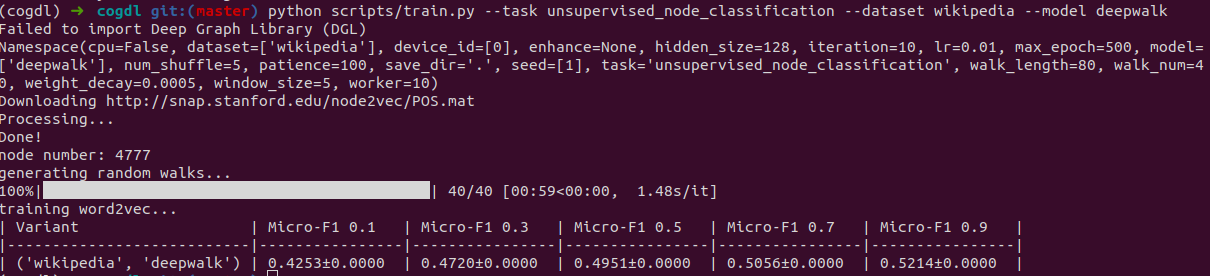
\includegraphics[width=15cm, height=5.5cm]{Figures/cmd1}
		\vspace{-0.7cm}
		\caption{Result of running the first script}
	\end{figure}

	\vspace{-0.4cm}
	\noindent Accordingly, the second script (python scripts/train.py --task node\_classification --dataset citeseer -- model gcn) analyzes the same task but for training and testing the GCN model on the citeseer dataset. The obtained results are demonstrated in the below figure (Figure 2).
	
	\begin{figure}[H]
		\centering
		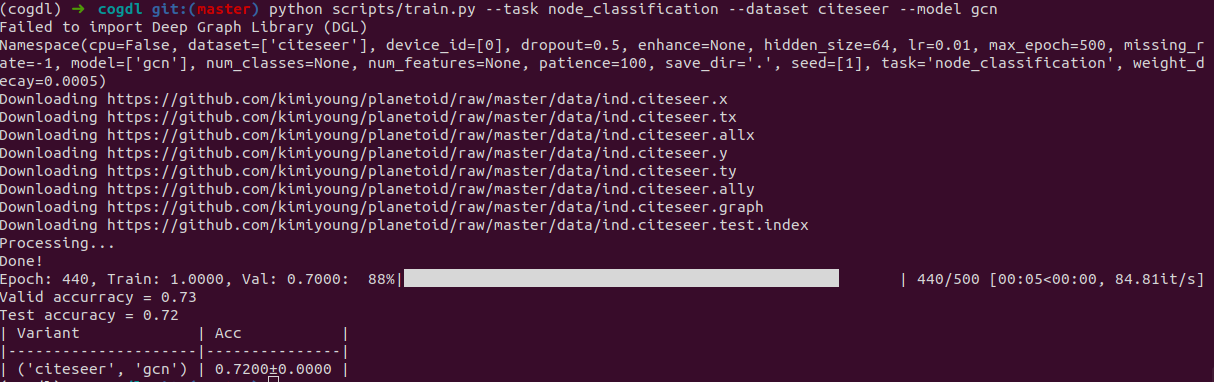
\includegraphics[width=15cm, height=6cm]{Figures/cmd2}
		\vspace{-0.7cm}
		\caption{Result of running the second script}
	\end{figure}
	
	\subsection{API Design}
	\noindent CogDL is a graph representation learning toolkit, based on PyTorch. Similar to what is demonstrated in the two scripts of the previous section, the main entry point of the model training is train.py located in the scripts folder. Initially, the arguments provided by the user are evaluated: first, it checks whether the provided arguments are valid; second, it checks whether the provided model matches the input task and dataset (based on match.yml file); third, the model implementation itself checks whether user provides all the required arguments.After the validity of the provided arguments is evaluated, CogDL checks whether the requested dataset is available offline. If this dataset has yet to be downloaded, the download script is called to download the corresponding datasets.
	
	\vspace{0.1cm}
	\noindent CogDL's API is fairly easy to use. First, setting the hyper-parameters for a specific model can be achieved by modifying the keys of 'args' variable, which is globally used in machine learning frameworks. For instance, for the task of graph classification, on the proteins dataset with the hgpsl model, we would have
	
	\vspace{-0.3cm}
	\begin{center}
		args = default\_args()\\
		args.task = 'graph\_classification'\\
		args.dataset = 'proteins'\\
		args.model = 'hgpsl'
	\end{center}

	\vspace{-0.2cm}
	\noindent In addition, the model and its dataset can be built via the following lines:
	
	\vspace{-0.2cm}
	\begin{center}
		dataset = build\_dataset(args)\\
		model = build\_model(args)\\
	\end{center}

	\vspace{-0.2cm}
	\noindent Consequently, we can create the task using the model and dataset and train it via
	
	\vspace{-0.2cm}
	\begin{center}
		task = build\_task(args, dataset=dataset, model=model)\\
		ret = task.train()\\
	\end{center}

	\vspace{-0.2cm}
	\noindent Each of the implemented models reside in the cogdl/nn folder. The structure of the models are somewhat similar: a sub-class of base model which has an 'add\_args' function to initialize its arguments, 'build\_model\_from\_args' function that builds the model based on those arguments, an init function to initialize and define the different layers and variables of the model structure, a forward function to demonstrate the feed forward operation of the model and its relative calculations, and occasionally, a loss and a predict function whose roles are believed to be self-explanatory. There are also different tasks and datasets within the cogdl folder. The task scripts are used to train, test, and evaluate models relative to the task while the dataset scripts download and process the corresponding dataset.
	
	\noindent Each model also has an example of its usage, similar to what was previously explained, in the examples folder. Accordingly, the unit tests for both the models and datasets are provided in tests folder. The model unit tests dedicate two functions to declaring the required args for the model and evaluating the model respectively. Accordingly, the unit tests are tested via Travis once they are added to GitHub repository.
	
		\vspace{-0.3cm}
	\subsection{GNN Model Implementation}
	
	\noindent In this assignment, I implemented the Hierarchical Graph Pooling with Structure Learning model [1]. The pull request id for this implementation is \href{https://github.com/THUDM/cogdl/pull/80}{\#80} and it has been merged at the time of writing this report.
	
		\vspace{-0.3cm}
	\subsection{Suggestions}
	\noindent There are a number of suggestions that I believe would improve the CogDL experience, both as a user and as a contributor:
	\begin{enumerate}
		\item Create a unified template for all the models for a certain tasks; this allows users to clearly differentiate between different models and provides contributors with a clear path to implement their models. 
		\item Include more information on how the evaluation results in the README.md file have been obtained. For instance, for tasks such as graph classification, there aren't any mentions of using k-folds or other arguments to make the models work on certain dataset; yet, these arguments are highly necessary.
		\item Make a list of content for the README. The current version of the README file looks rather complex, long, and hard to look through. Providing an interactive list of content would allow the users to focus on the topics of each section and find the section they are looking for much better and faster.
	\end{enumerate}
	
	\vspace{-0.5cm}
	\subsection{Contributions}
	
	\noindent As my contribution to this toolkit, I have made an interactive CLI to make the necessary files for a new model (check figure below).
	
	\begin{figure}[H]
		\centering
		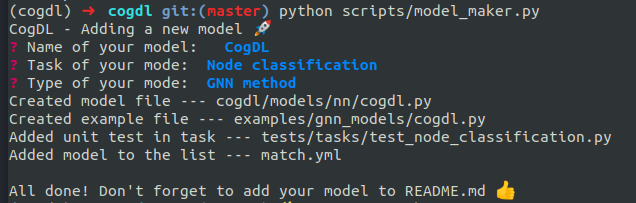
\includegraphics[width=15cm, height=5cm]{Figures/model}
		\vspace{-0.7cm}
		\caption{Model maker CLI}
	\end{figure}

	\vspace{-0.4cm}
	\noindent As shown in the figure, the script can be accessed by running 'python scripts/model\_maker.py'. The script then asks the user several questions to have the necessary information for creating a new file. Accordingly, the script does the following tasks based on user inputs:
	
	\begin{enumerate}
		\item Create a model file in the nn folder based on a predefined template.
		\item Create an example file in the corresponding folder of the model's type, according to a predefined template.
		\item Add the unit test for this model to the corresponding task.
		\item Add the model to the list of available models in math.yml.
		\item Remind the user to add their own model to README.md since the CLI is yet unavailable to detect the correct location to add the model. In addition, since the model is yet to be defined, its evaluation is not possible.
	\end{enumerate}

	\noindent The pull request id for this contribution is \href{https://github.com/THUDM/cogdl/pull/86}{\#86}  and it has been merged at the time of writing this report.
	
	\vspace{-0.4cm}
	\section*{References}
	[1] Zhen Zhang et al. “Hierarchical graph pooling with structure learning”. In: arXiv(2019) arXiv:1911.05954


	
\end{document}